



some introduction about our iso 14040..

\begin{comment}
\subsection{Goal of this LCA}
The purpose of this assessment and who are the results intended for, the audience of this study. 
Answer: This paper is comparing two different products that fulfills the same function which is simply exchange business card or business card information or exchange of business contact between two or more users. The purpose of using this study is marketing of the product also regulating the use of product. Furthermore we are not trying to identify the possible improvements for the existing products (such as paper based business card). This study is not meant to identify eco-label of the existing product paper business cards and the application. We are merely introducing a product that does similar function to existing paper based business card.

\subsection{The scope}
What is included in the system and what detailed assessment to be used in this study.
Since we are comparing two products we will have two system each with different boundaries. PBC has only one function which exchange of business card whereas our application or DBC can have multiple functionality such exchange, manage business cards, secure business cards exchange. Normally the only way to avoid multi-functionality of the product by allocation or division of the system based on its functionality as explained in cite{ekvall2001allocation} or dividing the system based on process (non-physical division). We have managed to avoid all the allocation and division problems which will be discussed in functional unit section. 
Some assumption about the PCB and DCB are given below 

\begin{itemize}
\item ABC
\item CDE
\end{itemize}


\subsection{Functional Units}
Functional unit defines the foundation of LCA for comparing two or more products. All data collected in the inventory will be dependent on this functional unit. For example when comparing plastic bag versus paper bag. The function of these products is to carry groceries, hence the functional unit will be volume of groceries. For instance one plastic bag carries twice the volume of groceries than paper bag. Since these products cannot contain same amount of grocery then they cannot be compared on 1 to 1 basis. Instead two paper bag will be determined as having equivalent function one plastic bag. In our case the both products can be compared on 1 to 1 basis because each exchange between two people contain will contain exchange of two cards or exchange of two packets of information in our application. Furthermore exchange between 3 people will require exchange of $3 x 2$ $(6)$ paper based business cards similarly exchange between 3 people using the app will require $3 x 2$ of packets of information delivered to app. In general if n people were to exchange business cards among themselves then it would require $n(n-1)$ exchanges. Hence we can assume that both products (paper based business card and app) can be compared on one to one basis. More importantly the exchange of PBC has zero impact on the environment because exchange two pieces of paper by two people is simply handing over the cards to each other while exchanging DBC requires generation of virtual packet and exchanged over the internet. In DBC the virtual packets are generated and exchanged on demand unlike PBC in which generating cards requires a lengthy process of formatting and printing. For the purpose of equal comparability we will take into consideration the environmental impact of generation and exchange of PBC and DBC. 
Most printing services produce minimum number of 50 cards per user and we need two users to exchange business cards with each other. More realistic scenario would be 50 user printing 50 cards each and exchanging $50 x 49$ times. In DBC system we can broadcast the single virtual packet that contains a user contact information to the 49 people surrounding him which is much more efficient method than one-to-one exchange. For simplicity we will only calculate the impact of 50 exchange between two users only for both systems because there is no such broadcast technique in PBC.

Other aspects that should be considered while comparing are 
\begin{itemize}
\item efficiency of the product, the paper based exchange is less efficient due to lacking broadcast, multicast techniques. Furthermore organizing and managing PBC is gets cluttered to fast because it requires manually indexing the cards, while DBC take care of such issues seamlessly. For performing LCA the application will not contain such features to for making the comparability fair.
\item the durability of the products, the paper based business card can be less durable because it depends on the physical degradation of the product on the other hand the business card information in app is virtual and can be more durable since it can be replicated or backed up easily with small cost.
\item The performance quality standard not decided yet.
\end{itemize}

For simplification purposes we are not examining any other functions of the products. The paper based business card has only one function to exchange cards, whereas app can have multiple functionality such as backup of cards on the cloud, broadcast and multicast techniques, secure card exchange, auto card information update and many other. For tackling such problems ISO has proposed obvious solution for subdividing the processes into separate process the ISO procedure (ISO 14041, 1998) \cite{ISO140402006} 
To make two products more comparable, in this study we will only perform LCA on app version which includes only single function of card exchange without other extra functions. Such app version is accessible to us because we are the core developer of the app. Most non-comparative ICT LCA avoided the problem of allocation and multi-functional product such as smart phone, laptop, PC and e-reader \cite{choi2006life,frey2006ecological,lu2006balancing}. In these studies the approach used by authors simplifies their study and hence these studies modified their LCA accordingly. In contrast, our app prototype will be singular function product. Therefore the complexity of allocation and multifunctional product will be avoided.


\subsection{System boundaries}

In our case the DBC doesn’t have any raw material as input to the system. Because all the coding comes from the user capabilities itself. The only energy consumed by production of the application are due the tools and facilities used by the developers, graphics designer and project manager. Figure depicts some of the facilities needed by developer this includes custom software such Eclipse IDE and energy needed to run PCs, Air Conditioner, UPS, heater, printer and many others that will be discussed in detail in coming section.


\begin{figure}[h]
\centering
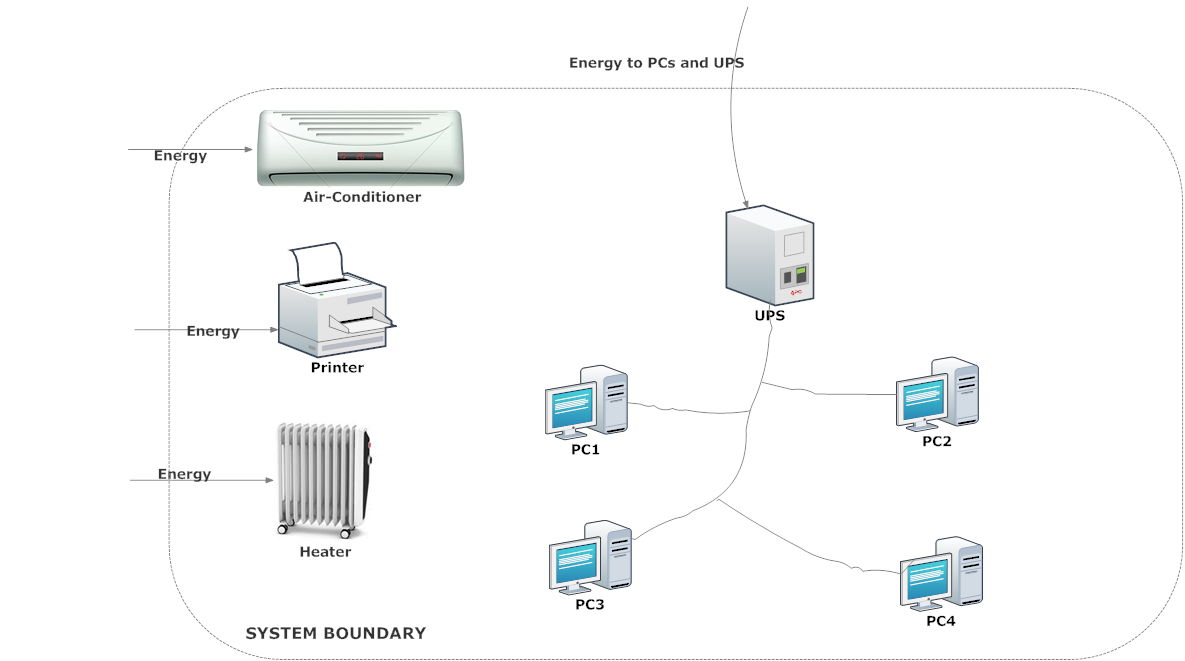
\includegraphics[width=8cm]{systemboundarycomprehensive.png}
\caption{System boundary of production phase of application }
\label{fig Milanmap}
\end{figure}



\begin{figure}[h]
\centering
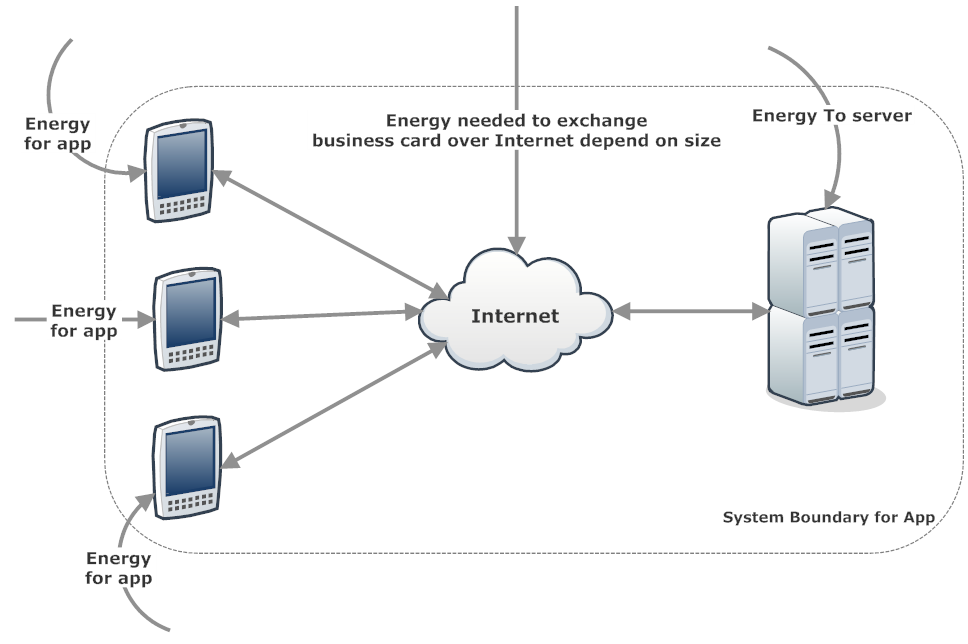
\includegraphics[width=8cm]{systemboundryICT.png}
\caption{Application (DBC) during use phase}
\label{fig Milanmap}
\end{figure}


\end{comment}